\documentclass[9pt,twoside,lineno]{pnas-new}
% Use the lineno option to display guide line numbers if required.

\templatetype{pnasmathematics} % Choose template 
% {pnasresearcharticle} = Template for a two-column research article
% {pnasmathematics} = Template for a one-column mathematics article
% {pnasinvited} = Template for a PNAS invited submission

\usepackage{algorithm}
\usepackage[noend]{algpseudocode}
\usepackage{subfig}
\graphicspath{{figures/}}
\DeclareMathOperator*{\argmax}{argmax}
\DeclareMathOperator*{\argmin}{argmin}
\newcommand{\norm}[1]{\left\lVert#1\right\rVert}

\title{Learning complex models with invertible neural networks: a likelihood-free Bayesian approach}

% Use letters for affiliations, numbers to show equal authorship (if applicable) and to indicate the corresponding author
\author[1]{Stefan T. Radev}
\author[1]{Ulf K. Mertens} 
\author[1]{Andreas Voss}
\author[2]{Lynton Ardizzone}
\author[2]{Ullrich Köthe}

\affil[1]{Institute of Psychology, Heidelberg University, Hauptstr. 47-51, 69117 Heidelberg, Germany}
\affil[2]{Heidelberg Collaboratory for Image Processing (HCI), Interdisciplinary Center for Scientific Computing (IWR), Heidelberg University, Im Neuenheimer Feld 205, 69120 Heidelberg, Germany}

% Please give the surname of the lead author for the running footer
\leadauthor{Radev} 

% Please add here a significance statement to explain the relevance of your work
\significancestatement{Describing complex stochastic processes with parametric  models lies at the heart of science. Simulating models given a set of parameters is relatively easy with the aid of modern computers, but inferring model parameters from observed data can often be a challenging endeavor. We combine recent advances in deep learning and Bayesian inference into a powerful method for building reusable parameter estimation networks applicable to various types of models and data encountered in different research fields.}

% Please include corresponding author, author contribution and author declaration information
\authorcontributions{Please provide details of author contributions here.}
\authordeclaration{This research was supported by the Deutsche Forschungsgemeinschaft (DFG, German Research Foundation; grant number GRK 2277 "Statistical Modeling in Psychology")}


\correspondingauthor{\textsuperscript{2}To whom correspondence should be addressed. E-mail: stefan.radev\@psychologie.uni-heidelberg.de}

% At least three keywords are required at submission. Please provide two to five keywords, separated by the pipe symbol.
\keywords{Deep learning $|$ Invertible networks $|$ Bayesian inference $|$ Parameter estimation $|$ Stochastic models} 

\begin{abstract}
Parametric models of complex processes are ubiquitous throughout the sciences. As the processes under study and the models describing them become increasingly complex, parameter estimation with standard Bayesian and frequentist methods can quickly become intractable. To address this, we propose a novel method for likelihood-free inference based on invertible neural networks. The method is capable of performing fast full Bayesian inference on large amounts of data by training the networks on simulated data and learning to invert the model under study. The method is independent of particular data formats, as it includes a summary network trained to embed the observed data into fixed-size vectors in a data-driven way. This makes the method applicable to various scenarios where standard inference techniques fail. We demonstrate the utility of the method on a toy model with known analytic posterior and on example models from population dynamics, epidemiology, cognitive science and genetics. We argue for a general framework for building reusable parameter estimation machines for potentially any process model from which simulations can be obtained.
\end{abstract}

\dates{This manuscript was compiled on \today}
\doi{\url{www.pnas.org/cgi/doi/10.1073/pnas.XXXXXXXXXX}}

\begin{document}

\maketitle
\thispagestyle{firststyle}
\ifthenelse{\boolean{shortarticle}}{\ifthenelse{\boolean{singlecolumn}}{\abscontentformatted}{\abscontent}}{}

\dropcap{M}athematical models are formal descriptions of scientific theories allowing a clear and unambiguous way to formulate and test scientific hypotheses about probabilistic phenomena in a probabilistic world. In its most abstract form, a mathematical model is specified by a set of parameters $\boldsymbol{\theta}$ and a forward model $q$ mimicking the process by which manifest data $\boldsymbol{x}$ arise from latent parameters: 
\begin{align*}
\boldsymbol{x}= q(\boldsymbol{\theta}) \numberthis \label{eqn:1} 
\end{align*}
While $q$ can represent an arbitrarily complex process by an arbitrarily complicated expression, its functional form is usually guided by a well-founded theoretical framework. For instance, $q$ can be a stochastic differential equation describing the dynamics of single neurons in the brain, or a step-by-step biological algorithm dictating the rate of gene expression in certain cells. Thus, it is only through theoretical embedding that a meaningful interpretation in terms of some mechanism can be attached to the parameters of a mathematical model. Examples of mathematical models can be found in various scientific domains, e.g., genetics \cite{zappia2017splatter, beaumont2002approximate}, cognitive science \cite{palestro2018likelihood, usher2001time}, neuroscience \cite{hwang2018conditional, lueckmann2017flexible}, population dynamics \cite{wood2010statistical}, epidemiology \cite{keeling2011modeling,hethcote2000mathematics}, just to name a few.

Once a mathematical model has been formulated, the next step consists of fitting the model to experimental or observational data and recovering the parameters of interest. However, estimating the parameters of a mathematical model from data can quickly become one of the most tenacious challenges in applications to real-world problems. It is also one of the most important ones to be tackled, since without reliable parameter estimation methods, it is impossible to test the utility of a model, regardless of its sophistication or theoretical appeal. Idealized parameter estimation involves computing the inverse (backward) model $\boldsymbol{\theta} = q^{-1}(\boldsymbol{x})$ exactly. However, due to noise, inherent stochasticity or loss of information, the inverse usually does not exist, so researchers need to resort to the sophisticated frameworks of Bayesian or frequentist inference. 

However, as mathematical models and processes under description become increasingly complex, parameter estimation and model selection can quickly become intractable with standard Bayesian and frequentist method. Complex models specified by a generative stochastic mechanism do not always provide a closed-form solution for the \textit{likelihood function} \cite{palestro2018likelihood, csillery2010approximate, toni2009simulation}. This poses great difficulties for Bayesian and frequentist methods alike, since both depend explicitly on the numerical evaluation of a likelihood function as a proxy for assessing model fit to data. Even if a likelihood function is available in closed-form, inference may be prohibitively slow for real-world applications. In this case, enforcing simplifying distributional assumptions (i.e., independence or Gaussian assumptions) on the likelihood can increase the speed of inference, but can also lead to model misspecifications and dramatically incorrect estimates. Therefore, the need for powerful and reliable likelihood-free estimation methods arises naturally. 

Likelihood-free methods aim at bypassing the above problems by resorting to a simulation-based approach to parameter estimation and model selection \cite{palestro2018likelihood, turner2014generalized}. A subset of likelihood-free methods includes approximate Bayesian computation (ABC) methods, which aim at preserving the advantages of Bayesian data analysis even when the likelihood function is intractable or practically impossible to compute \cite{turner2014generalized, sunnaaker2013approximate, csillery2010approximate}. ABC methods approximate the likelihood function by repeatedly sampling parameters from a pre-specified prior distribution $p(\boldsymbol{\theta})$ and then simulating multiple datasets by running the generative model $q(\boldsymbol{\theta})$ using the sampled parameters. Thus, the core ingredients of ABC methods are a prior on $\boldsymbol{\theta}$, and a generative model $q(\boldsymbol{\theta})$, usually specified as a function code in a general-purpose programming language \cite{csillery2010approximate, mertens2018abrox}.

Performing approximate inference comes at the cost of incurring additional approximation error, which accumulates on top of the irreducible estimation error. Within the context of approximate inference, the most common manifestations of approximation error include: \textit{i)} imprecise form of the posterior; \textit{ii)} imprecise posterior moments; \textit{iii)} under- or overestimation of uncertainty. Different approximation methods usually involve multiple trade-offs between minimizing approximation error and keeping computational time within reasonable bounds \cite{frazier2018asymptotic, palestro2018likelihood}.

Recently, ideas from machine learning and deep learning research have entered the field of likelihood-free inference in an attempt to overcome some of the shortcomings of traditional methods \cite{radev2019towards, hwang2018conditional, mestdagh2018prepaid, raynal2018abc, jiang2017learning, lueckmann2017flexible, papamakarios2016fast}. The most common approach has been to cast the problem of parameter estimation as a supervised learning task. In this setting, a large dataset of the form $\boldsymbol{D} = \{h(\boldsymbol{x}^{(i)}), \boldsymbol{\theta}^{(i)}\}_{i=1}^{n}$ is created by repeatedly sampling from $p(\boldsymbol{\theta})$ and simulating an artificial dataset $\boldsymbol{x}$ by running $q(\boldsymbol{\theta})$ with the sampled parameters. Usually, the dimensionality of the simulated data is reduced by computing summary statistics  with a fixed summary function $h(\boldsymbol{x})$. Then, a supervised learning algorithm $f(h(\boldsymbol{x});\boldsymbol{\phi}) = \widehat{\boldsymbol{\theta}}$ with learnable parameters $\boldsymbol{\phi}$ (e.g., linear regression, random forest, neural network) is trained on the simulated data to later output an estimate of the true data generating parameters. Thus, $f(h(\boldsymbol{x});\boldsymbol{\phi})$ essentially attempts to “learn” the intractable inverse model $\boldsymbol{\theta} = q^{-1}(\boldsymbol{x})$.

Inspired by previous machine learning approaches, the current work proposes a novel and universal likelihood-free method capable of performing full Bayesian inference on any mathematical process model from which simulations can be obtained. It treats parameter inference as a task of inverting a generative model and achieves this by drawing on the modern framework of deep probabilistic modeling for tackling intractable posteriors \cite{ardizzone2018analyzing, kingma2018glow, grover2018flow, dinh2016density}. The method integrates two separate deep neural networks modules (detailed in the \textbf{Methods} section) trained jointly on simulated data: a \textit{summary network} and an \textit{invertible network}. 

The \textit{summary network} is responsible for learning the most informative summary statistics directly from data. It should be designed to follow the functional and probabilistic symmetries inherent in the data, e.g. a permutationally invariant network for \textit{i.i.d.} data \cite{bloem2019probabilistic}, a recurrent network for time-series data, or a convolutional network for grid-like data \cite{goodfellow2016deep}. The computation of summary statistics is a crucial aspect in likelihood-free inference. Previous approaches mainly use hand-crafted summary statistics tailored to the specific application. However, in many application, it is not straightforward to settle upon a set of good summary statistics. Thus, the summary network completely eliminates the need to manually specify a fixed number of summary statistics and makes the method independent of the format or the size of the data.

The \textit{invertible network} is responsible for learning the posterior of the model parameters given the observed and summarized data. It is based on the recently developed flow-based architecture \cite{kingma2018glow, grover2018flow, dinh2016density}. Flow-based methods provide exact latent-variable inference and log-likelihood evaluation when operating at optimum. In the \textbf{Methods} section, we show that our method maximizes the posterior over model parameters directly when cast in the context of likelihood-free inference. Furthermore, flow-based methods are capable of approximating very high-dimensional distributions (e.g., the pixels of an image). Once trained with a sufficient amount of simulated data, our invertible network can perform full Bayesian inference on large amounts of real data from a given domain in a single pass. 

\begin{figure}
    \centering
    \subfloat[Training phase]{{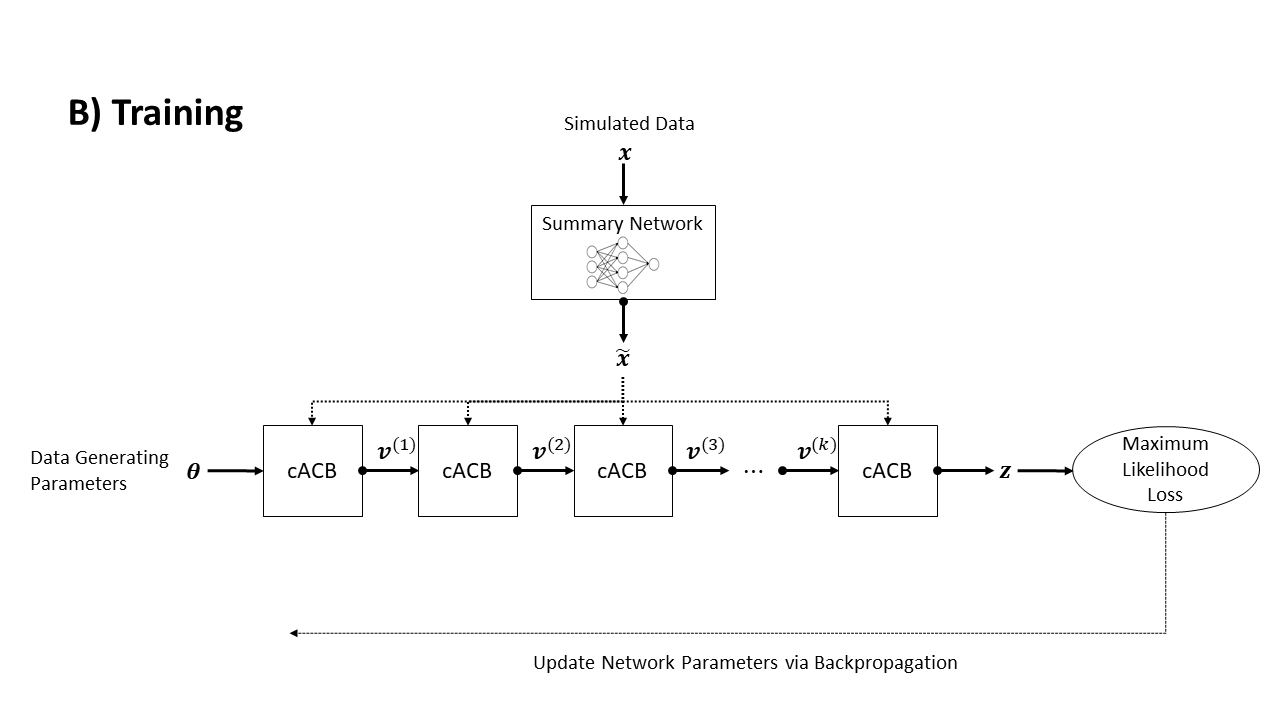
\includegraphics[width=.99\linewidth]{training.png}}}
    \newline
    \subfloat[Inference phase]{{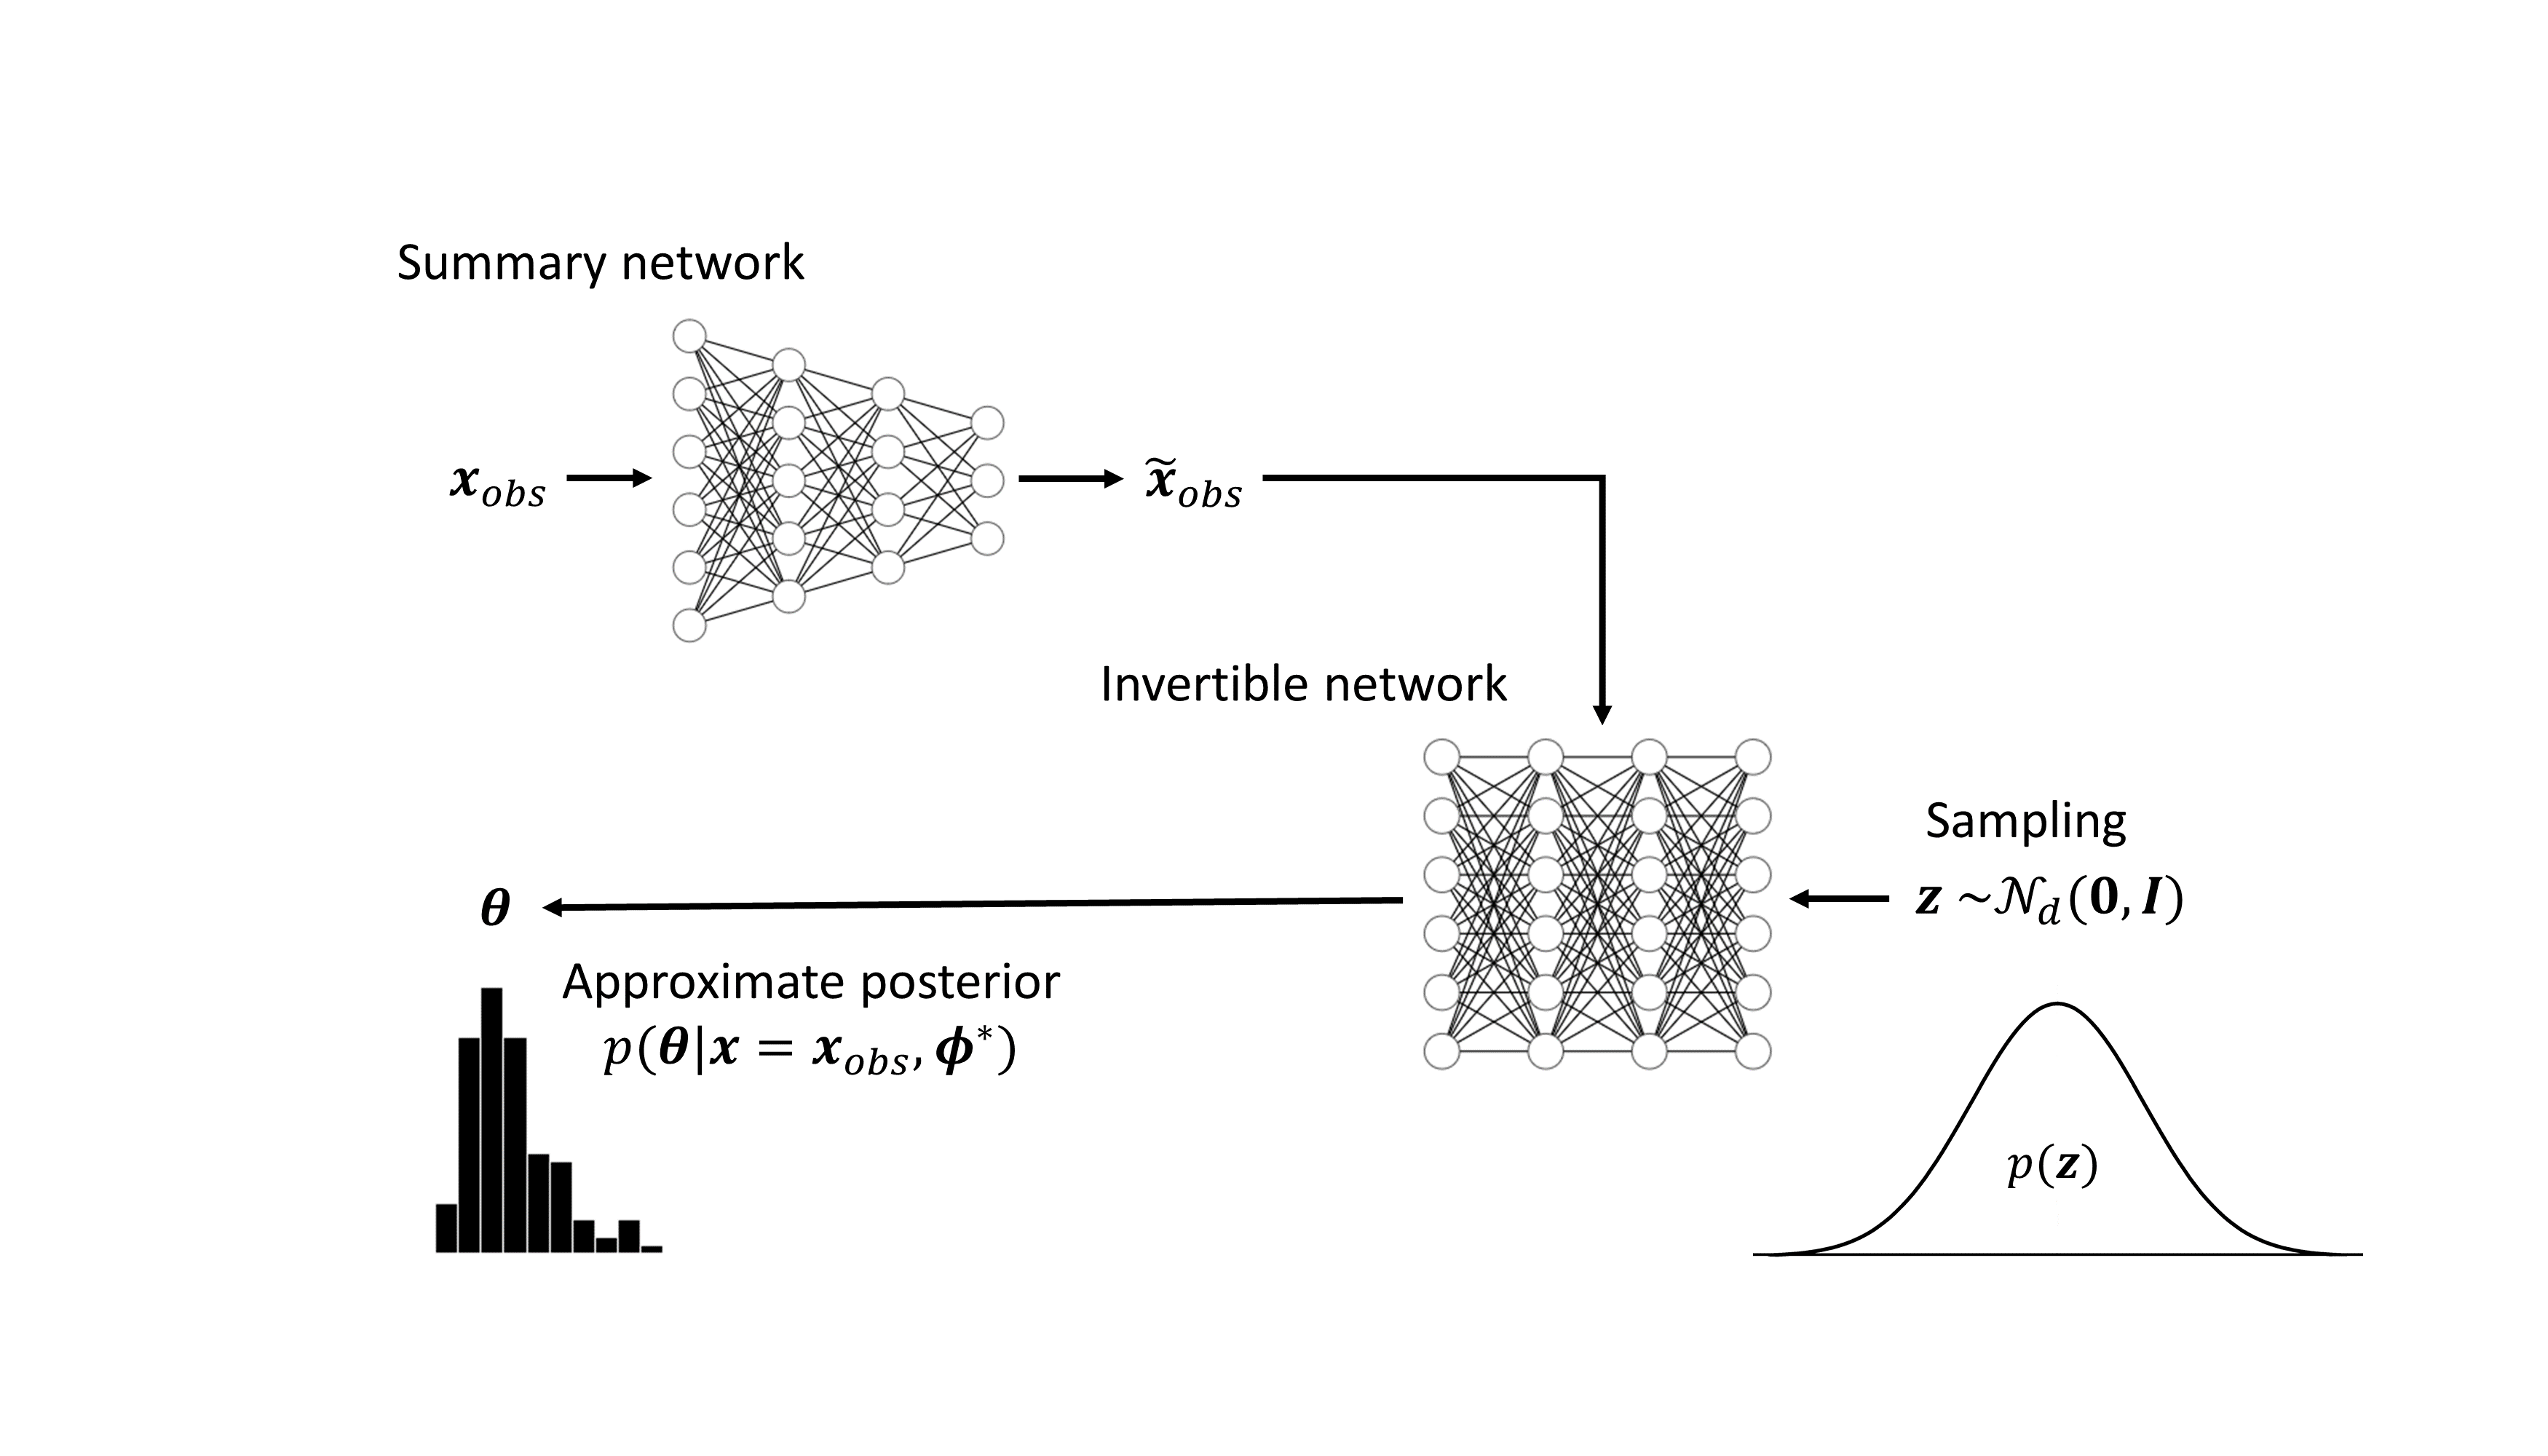
\includegraphics[width=.99\linewidth]{inference.png}}}
    \caption{A graphic illustration of the two phases of the method. \textbf{(a)} During the training phase, the networks are trained on simulated data from the model; \textbf{(b)} during the inference phase, the true posterior of the model parameters is approximated from real data.}
    \label{fig:first}
\end{figure}

The joint training of a summary network and an invertible network results in a powerful and universal parameter estimation machine capable of inverting complicated statistical problems in various scientific domains (see Fig.1). Moreover, the method addresses many of the limitations of previous likelihood-free methods. First, it involves no costly MCMC or rejection sampling, which makes the inference phase lightning fast, as we also make use of GPU-accelerated computation. Second, it involves no fixed summary statistics or kernels, but learns the most informative representation of the data in an end-to-end manner. Third, the method is fully Bayesian, as it directly learns the posterior over model parameters and thus allows for the quantification of uncertainty, which is a crucial requirement in parameter estimation \cite{kendall2017uncertainties, gelman2013bayesian}. Last, the trained networks can be shared and reused by multiple researches within a scientific domain, thus removing the need for wasteful computations and fitting a separate model for each and every dataset. This pooling of computational resources across researches is an important step forward in mathematical modeling, as has been recently argued \cite{mestdagh2018prepaid}.

To illustrate the utility of the new method, we first apply it to a toy Bayesian regression model with known posterior. Then, we present applications to intractable models from cognitive science, population dynamics, epidemiology, and genetics and demonstrate state-of-the art parameter recovery. The outline of the remaining manuscript is as follows: The \textbf{Methods} section introduces the main building blocks of the new method and summarizes the main steps as pseudocode. The \textbf{Results} section presents the various applications of the model to real-world research domains. Finally, the \textbf{Discussion} section lists the advantages of the current method, treats some potential pitfalls and explores future research vistas. Python code and data for all applications are freely available as Jupyter notebooks at \href{https://github.com/stefanradev93/cINN}{https://github.com/stefanradev93/cINN} and as a small library based on \textit{TensorFlow} \cite{abadi2016tensorflow} for creating and training custom invertible networks with GPU-support. 

\section*{Methods}

\subsection*{Notation}

In the following, we denote observed or simulated univariate datasets from the mathematical model of interest as $\boldsymbol{x} = (x_{1}, x_{2},...,x_{n})$, and multivariate datasets as $\boldsymbol{X} = (\boldsymbol{x}_{1}, \boldsymbol{x}_{1},...,\boldsymbol{x}_{n})$. The parameters of a mathematical model are represented as a vector $\boldsymbol{\theta} = (\theta_{1}, \theta_{2},...,\theta_{d})$, and all trainable parameters of the invertible and summary neural networks as $\boldsymbol{\phi} = (\boldsymbol{\phi}_{inv}, \boldsymbol{\phi}_{sum})$. The number of parameters of a mathematical model will be denoted as $d$, and the number of simulated data points as $n$.

\subsection*{Deep Probabilistic Modeling}

Our method draws on major advances in modern deep probabilistic modeling, also referred to as deep generative modeling \cite{bloem2019probabilistic, kingma2018glow, ardizzone2018analyzing, kingma2014auto}. A hallmark idea in deep probabilistic modeling is to handle intractable target probability distributions by sampling from simpler distributions (e.g., Gaussian or uniform distributions) and transforming these samples via a complex non-linear, learnable transformations. Most popular deep probabilistic models entail two phases. During the \textit{training phase}, a transformation from the simple to the desired target distribution is learned by optimizing a cost function via backpropagation. During the \textit{inference phase}, samples from the target distribution are obtained by sampling from the simple distribution and applying the transformation learned during the training phase. Using this approach, recent applications of deep probabilistic models have achieved unprecedented results on extremely high-dimensional and intractable problems (e.g., complex data distributions such as natural images, music, or text).

In the context of mathematical modeling and Bayesian inference, the target distribution is the posterior distribution of model parameters $p(\boldsymbol{\theta}|\boldsymbol{x})$ capturing our uncertainty about the numerical values of parameters given empirical data. We can leverage the fact that most mathematical models are generative in nature and as such can be used to perform multiple simulations of the process of interest. By specifying a prior distribution over the model parameters $p(\boldsymbol{\theta})$, one can generate arbitrarily large datasets of the form $\boldsymbol{D} = \{\boldsymbol{x}^{(i)}, \boldsymbol{\theta}^{(i)}\}_{i=1}^{n}$ and use a deep generative model to learn a probabilistic mapping from data to parameters. Thus, at inference time, one can condition the model on observed data $\boldsymbol{x}_{obs}$ and obtain samples $\boldsymbol{\theta}_{1}, \boldsymbol{\theta}_{2},...,\boldsymbol{\theta}_{L}$  approximating the posterior $p(\boldsymbol{\theta}|\boldsymbol{x}=\boldsymbol{x}_{obs})$ in the manner described above.

In the current work, we propose to implement and use a conditional invertible neural network (cINN) architecture. Previously, INNs have been successfully employed to model data from astrophysics and medicine\cite{ardizzone2018analyzing}. We adapt the model to suit the task of parameter estimation in the context of mathematical modeling (see Figure 1 for a full graphical illustration of the method) and develop a reusable probabilistic architecture for full Bayesian likelihood-free inference on complex mathematical models.

\subsection*{The Affine Coupling Block}

The basic building block of a cINN is the affine coupling block (ACB) \cite{ardizzone2018analyzing, kingma2018glow, dinh2016density}. Each ACB consists of four separate fully connected neural networks denoted as $s_{1}(\cdot), s_{2}(\cdot), t_{1}(\cdot), t_{2}(\cdot)$. An ACB is specifically designed to be invertible, which means that in addition to a parametric mapping $f_{\boldsymbol{\phi}_{inv}}: \mathbb{R}^{d} \rightarrow \mathbb{R}^{d}$ it also learns the inverse mapping $f_{\boldsymbol{\phi}_{inv}}^{-1}: \mathbb{R}^{d} \rightarrow \mathbb{R}^{d}$ "for free". Denoting the input vector of $f_{\boldsymbol{\phi}_{inv}}$ as $\boldsymbol{u}$ and the output vector as $\boldsymbol{v}$, it follows that $f(\boldsymbol{u}; \boldsymbol{\phi}_{inv}) = \boldsymbol{v}$ and $f^{-1}(\boldsymbol{v}; \boldsymbol{\phi}_{inv}) = \boldsymbol{u}$. Invertibility is achieved by splitting the input vector into two parts $\boldsymbol{u} = (\boldsymbol{u}_{1}, \boldsymbol{u}_{2})$ and performing the following operations on the split input:
\begin{align*} 
\boldsymbol{v}_{1} &= \boldsymbol{u}_{1} \odot \exp(s_{1}(\boldsymbol{u}_{2})) + t_{1}(\boldsymbol{u}_{2}) \numberthis \label{eqn:2}  \\ 
\boldsymbol{v}_{2} &= \boldsymbol{u}_{2} \odot \exp(s_{1}(\boldsymbol{v}_{1})) + t_{1}(\boldsymbol{v}_{1}) \numberthis \label{eqn:3} 
\end{align*}
The outputs $\boldsymbol{v} = (\boldsymbol{v}_{1}, \boldsymbol{v}_{2})$ are then concatenated again and passed to the next ACB. The inverse operation is given by:
\begin{align*} 
\boldsymbol{u}_{2} &= (\boldsymbol{v}_{2} - t_{2}(\boldsymbol{v}_{1})) \odot \exp(-s_{2}(\boldsymbol{v}_{1})) \numberthis \label{eqn:4}  \\ 
\boldsymbol{u}_{1} &= (\boldsymbol{v}_{1} - t_{1}(\boldsymbol{u}_{2})) \odot \exp(-s_{1}(\boldsymbol{u}_{2})) \numberthis \label{eqn:5} 
\end{align*}
An additional property of this design, which becomes relevant later for optimization, is that the operations of the ACB have tractable, and cheaply computable Jacobians (strictly upper or lower triangular matrices). Furthermore, the internal networks $s_{1}(\cdot), s_{2}(\cdot), t_{1}(\cdot), t_{2}(\cdot)$ can be represented by arbitrarily complex neural networks, which themselves need not be invertible, since they are only ever evaluated in the forward direction during both the forward and the inverse pass through the ACB. To ensure that the model is powerful enough to represent complicated distributions, we chain multiple ACBs, so that the output of each ACB becomes the input of the next. In this way, the whole chain remains invertible from the first input to the last output and can be viewed as a single function parameterized by trainable parameters $\boldsymbol{\phi}_{inv}$.

In our applications, the input to the first ACB is the parameter vector $\boldsymbol{\theta}$, and the output of the final ACB, denoted hitherto as $\boldsymbol{z}$, is encouraged to follow a $d$-dimensional spherical Gaussian via optimization (described in detail later), that is, $p(\boldsymbol{z}) = \mathcal{N}_{d}(\boldsymbol{z}|\boldsymbol{0},\boldsymbol{I})$. Fixed permutation matrices are used before each ACB to ensure that each axis of the latent space encodes information from all components of $\boldsymbol{\theta}$. In order to take into account the observed data $\boldsymbol{x}$, each of the internal networks of each ACB is augmented to take $\boldsymbol{x}$ as an additional input - $s_{1}(\cdot,\boldsymbol{x}), s_{2}(\cdot,\boldsymbol{x}), t_{1}(\cdot,\boldsymbol{x}), t_{2}(\cdot,\boldsymbol{x})$ - so a complete pass through the entire invertible chain can be expressed as:
\begin{align*} 
f(\boldsymbol{\theta};\boldsymbol{x},\boldsymbol{\phi}_{inv}) = \boldsymbol{z} \numberthis \label{eqn:6}
\end{align*}
together with the inverse operation:
\begin{align*} 
f^{-1}(\boldsymbol{z};\boldsymbol{x},\boldsymbol{\phi}_{inv}) = \boldsymbol{\theta} \numberthis \label{eqn:7}
\end{align*}

This process can be interpreted as follows: the forward pass maps data-generating parameters to $\boldsymbol{z}$-space using conditional information of $\boldsymbol{x}$, while the inverse pass maps data points from $\boldsymbol{z}$-space to the data-generating parameters of interest using the same conditional information provided by the data. In the next section, we describe the optimization procedure used to match the outputs of $f^{-1}(\boldsymbol{z};\boldsymbol{x},\boldsymbol{\phi}_{inv})$ to the posterior $p(\boldsymbol{\theta}|\boldsymbol{x})$.

\subsection*{Summary Network}
Since in practice the conditioning data set $\boldsymbol{x}$ can have variable number of input points (e.g., trial sizes, time points) and exhibit various redundancies, the cINN can profit from some form of dimensionality reduction applied to the data. Ideally, we want to avoid hand-crafted summary statistics, and instead learn the most informative summary statistics directly from data. Therefore, instead of feeding the raw simulated (observed) data to each ACB, we pass the data through an additional summary network to obtain a fixed-sized vector of learned summary statistics $\tilde{\boldsymbol{x}} = h(\boldsymbol{x};\boldsymbol{\phi}_{sum})$ and learn the parameters of the summary network $h$ jointly with those of the cINN chain via backpropagation. Thus, the current method remains completely end-to-end and is capable of generalizing to data sets of variable input size and structure.

\subsection*{Learning the Posterior}
The cINN learns to approximate the posterior of model parameters by optimizing  a maximum likelihood (ML) criterion. Broadly speaking, the goal of ML estimation is to find a set of parameters which maximize the probability of the data under a parametric model. In our case, we are interested in maximizing the expectation over possible neural network parameters with respect to the parameters of the mathematical model:
\begin{align*} 
\boldsymbol{\phi}^{*} = \argmax_{\boldsymbol{\phi}}\mathbb{E}_{\boldsymbol{\theta} \sim p(\boldsymbol{\theta}|\boldsymbol{x})}\left[p(\boldsymbol{\phi}|\boldsymbol{\theta},\boldsymbol{x})\right] \numberthis \label{eqn:8}
\end{align*}
Applying Bayes' rule to the posterior over all neural network parameters we obtain:
\begin{align*} 
p(\boldsymbol{\phi}|\boldsymbol{\theta},\boldsymbol{x}) \propto p(\boldsymbol{\theta}|\boldsymbol{x},\boldsymbol{\phi})p(\boldsymbol{\phi})  \numberthis \label{eqn:9}
\end{align*}
Note, that by maximizing eq.\ref{eqn:9} we are maximizing the posterior over model parameters of interest $p(\boldsymbol{\theta}|\boldsymbol{x},\boldsymbol{\phi})$. Thus, it remains to find a tractable expression for eq.\ref{eqn:8} to be minimized by backpropagation given a finite number of simulated samples from the model. To this end, we recall that we can relate the pdf of $\boldsymbol{\theta}$ to that of $\boldsymbol{z}$ via the change of variable theorem:
\begin{align*} 
p(\boldsymbol{\theta}|\boldsymbol{x},\boldsymbol{\phi}) &= p(\boldsymbol{z})\left|\det\left(\frac{\partial \boldsymbol{z}}{\partial \boldsymbol{\theta}}\right)\right| \numberthis \label{eqn:10} \\ 
&= p\left(f(\boldsymbol{\theta};\boldsymbol{x},\boldsymbol{\phi})\right)\left|\det\left(\frac{\partial f}{\partial \boldsymbol{\theta}}\right)\right| \numberthis \label{eqn:11}
\end{align*}
where $\partial f/\partial \boldsymbol{\theta} = \boldsymbol{J}_{f}$ is the Jacobian of the learned transformation $f(\boldsymbol{\theta};\boldsymbol{x},\boldsymbol{\phi})$ with respect to the input. Both terms in eq.\ref{eqn:11} are now tractable, since we have previously defined $\boldsymbol{z}$ as following a spherical unit Gaussian, that is, $p(\boldsymbol{z}) = (2\pi)^{-2/d}\exp(\norm{\boldsymbol{z}}_{2}^{2})$ and the log determinant of the Jacobian is easily computed as $s_{1}(\boldsymbol{u}_{2}, \boldsymbol{x}) + s_{2}(\boldsymbol{v}_{1}, \boldsymbol{x})$ due to eqs. \ref{eqn:2} and \ref{eqn:3}. We can now formulate the ML loss as the Monte-Carlo approximation of the negative logarithm of eq.\ref{eqn:8} for a batch of size $m$:
\begin{align*}
\mathcal{L}(\boldsymbol{\phi}) &= -\frac{1}{m}\sum_{i=1}^{m}\log\left(p(\boldsymbol{\phi}|\boldsymbol{\theta}^{(i)},\boldsymbol{x}^{(i)})\right) \numberthis \label{eqn:12} \\
&= -\frac{1}{m}\sum_{i=1}^{m}\log\left(p(\boldsymbol{\theta}^{(i)}|\boldsymbol{x}^{(i)},\boldsymbol{\phi})p(\boldsymbol{\phi})\right) \numberthis \label{eqn:13} \\
&= -\frac{1}{m}\sum_{i=1}^{m}\left(\frac{\norm{f(\boldsymbol{\theta}^{(i)};\boldsymbol{x}^{(i)},\boldsymbol{\phi})}_{2}^{2}}{2} + \log\left|\det\left(\boldsymbol{J}_{f}^{(i)}\right)\right|\right) + \tau\norm{\boldsymbol{\phi}}_{2}^{2} \numberthis \label{eqn:14}
\end{align*}
where we place a Gaussian prior over the neural network parameters with $\tau\equiv 1/\sigma^{2}$, corresponding to a standard $L2$-regularization.

Minimizing eq. \ref{eqn:14} can be interpreted as searching for the optimal neural network parameters $\boldsymbol{\phi}^{*}$ which maximize the probability of model parameters $\boldsymbol{\theta}$ given data $\boldsymbol{x}$. This is exactly the probability we are concerned with in Bayesian inference. Note that our formulation maximizes the posterior of model parameters directly, in contrast to variational methods which optimize a lower bound on the posterior \cite{papamakarios2016fast, kingma2014auto}.
Once the backpropagation algorithm has settled to a local minimum of the ML loss, one can easily obtain samples from the approximate posterior $p(\boldsymbol{\theta}|\boldsymbol{x}=\boldsymbol{x}_{obs},\boldsymbol{\phi}=\boldsymbol{\phi}^{*})$, based on an observed dataset $\boldsymbol{x}_{obs}$, by repeatedly sampling $\boldsymbol{z}^{(l)} \sim \mathcal{N}_{d}(\boldsymbol{0},\boldsymbol{I})$, and then passing $\boldsymbol{z}^{(l)}$ in reverse to the cINN in order to compute $\boldsymbol{\theta}^{(l)} = f^{-1}(\boldsymbol{z}^{(l)};\boldsymbol{x}_{obs},\boldsymbol{\phi}^{*})$ for $l=1,...,L$. Figure 1b illustrates the inference phase of the method. It is worth noting that sampling a large number of parameter values from the approximate posterior takes a negligible amount of time, since it only requires a single pass through the cINN in reverse.
 
\subsection*{Training the Networks}
We train all cINNs and summary networks described in this paper jointly via backpropagation. For all following experiments, we use the Adam optimizer  with a starter learning rate of $10^-3$ and an exponential decay rate of $.95$. We set the weight regularization parameter $\tau$ to a value of $10^{-5}$. We perform $100000$ iterations (network updates) for each of the examples in this paper, and report the results on the trained network. Note, that we did not perform an extensive search for optimal values of the cINN hyperparameter but use a cINN with 10 ACBs for each example in this paper (see \textbf{SI} for details of the cINN).
Concerning the data generation step, we use two training approaches. The first follows the classical approximate Bayesian computation approach to create a large “reference table” or grid of the form $\boldsymbol{D} = \{\boldsymbol{x}^{(i)}, \boldsymbol{\theta}^{(i)}\}_{i=1}^{n}$. The reference table is then used as training data for the neural network and training continues for a pre-specified number of epochs through the entire reference table. A separate validation dataset is eventually used to assess the performance of the network. This training approach separates the simulation from the training phase but can incur large memory overhead, as the reference table must be stored on disk and then loaded in chunks or in its entirety into memory. The second approach follows a different strategy, which is used mainly in the field of active learning. Correspondingly, a dataset, or a batch of datasets, is created on the fly and then passed through the neural network. This training regime has the advantage that the network never “experiences” the same input data twice. Moreover, training can continue as long as the network keeps improving (i.e., the loss keeps decreasing), since overfitting in the classical sense is nearly impossible. However, if the simulations are computationally expensive and researchers need to experiment with multiple models, it might be beneficial to switch to the first regime, since simulation and training in the active learning regime are tightly intertwined. TODO - Describe for which!

\subsection*{Putting It All Together}

On an abstract level, our method requires three key ingredients: 1) a mathematical process model $q(\boldsymbol{\theta})$ capable of simulating data $\boldsymbol{x}$; 2) a prior distribution over the model parameters $p(\boldsymbol{\theta})$ encoding our prior beliefs about plausible parameter values; 3) an invertible neural network $f_{\boldsymbol{\theta}}$ capable of approximating a large enough family of probability distributions (see Figure 2). In practice, a chain of up to 10 ACBs should suffice to learn most distributions encountered in the life sciences, since they tend to be unimodal and relatively simple (in contrast to the distribution of natural images or words in a spoken language). From these three ingredients, a universal and reusable sampler can be designed for likelihood-free Bayesian estimation of both tractable and intractable mathematical models. \textbf{Algorithm} \ref{Algorithm:algo} describes the essential steps of the method using an arbitrary summary network and employing the active learning training regime.

\begin{algorithm}
\caption{Bayesian likelihood-free inference with invertible neural networks}\label{Algorithm:algo}
\begin{algorithmic}[1]
\State \emph{Training (via active learning):}
\Repeat
\State {Sample a batch of $\{\boldsymbol{\theta}^{(i)}\}_{i=1}^{m}$ from prior $p(\boldsymbol{\theta})$}
\State {Simulate a batch of datasets $\{\boldsymbol{x}^{(i)}\}_{i=1}^{m}$ by running $\boldsymbol{x}^{(i)} = q(\boldsymbol{\theta}^{(i)})$ for $i=1,...,m$}
\State {Pass $\{\boldsymbol{x}^{(i)}\}_{i=1}^{m}$ through summary network $h(\boldsymbol{x}^{(i)};\boldsymbol{\phi}_{sum})$ to obtain $\{\tilde{\boldsymbol{x}}^{(i)}\}_{i=1}^{m}$}
\State {Pass $\{\boldsymbol{\theta}^{(i)}\}_{i=1}^{m}$ and $\{\tilde{\boldsymbol{x}}^{(i)}\}_{i=1}^{m}$ through cINN $f(\boldsymbol{\theta}^{(i)};\boldsymbol{x}^{(i)},\boldsymbol{\phi}_{inv})$ to obtain $\{\boldsymbol{z}^{(i)}\}_{i=1}^{m}$}
\State {Compute ML loss $\mathcal{L}(\boldsymbol{\phi})$ according to eq.\ref{eqn:14}}
\State {Update neural network parameters $\boldsymbol{\phi}$ via backpropagation}
\Until {convergence to $\boldsymbol{\phi}^{*}$}
\State \emph{Inference (given observed or test data $\boldsymbol{x}_{obs}$):}
\State {Summarize the observed data by computing $\tilde{\boldsymbol{x}}_{obs} = h(\boldsymbol{x}_{obs},\boldsymbol{\phi}_{sum}^{*})$}
\For{$l = 1,...,L$}
\State {Sample $\boldsymbol{z}^{(l)} \sim \mathcal{N}_{d}(\boldsymbol{0},\boldsymbol{I})$}
\State {Compute $\boldsymbol{\theta}^{(l)} = f^{-1}(\boldsymbol{z}^{(l)};\tilde{\boldsymbol{x}}_{obs},\boldsymbol{\phi}_{inv})$}
\EndFor
\State {\textbf{end for}}
\State {Use $\{\boldsymbol{\theta}^{(l)}\}_{l=1}^{L}$ to approximate the posterior $p(\boldsymbol{\theta}|\boldsymbol{x}_{obs})$}
\end{algorithmic}
\end{algorithm}

The backpropagation algorithm works by computing the gradients of the loss function w.r.t. the parameters of the neural networks and then adjusting the parameters, so as to drive the loss function to a local minimum. We experienced no instability or convergence issues during training with the ML loss. Note, that steps $12-15$ of \textbf{Algorithm} \ref{Algorithm:algo} can be executed in parallel with GPU support. 

In what follows, we apply the method to a toy Bayesian regression example with conjugate priors, and then use it to estimate the parameters of various intractable models from TODO -which?. Code for reproducing the results on all following examples is freely available at: \href{https://github.com/stefanradev93/cINN}{https://github.com/stefanradev93/cINN}.All examples are implemented in Python using the \textit{TensorFlow} library for automatic differentiation with GPU support.

\section*{Results}

\subsection*{Toy Example – Bayesian Regression}

As a proof-of-concept, we demonstrate the utility of our method in recovering the true analytic posteriors of the regression coefficients of a conjugate Bayesian regression model. To set the setting, assume we have observed a dataset $\boldsymbol{D} = \{(\boldsymbol{x}^{(i)},y^{(i)})\}_{i=1}^{n}$ with $\boldsymbol{x} \in \mathbb{R}^{d}$ and $y \in \mathbb{R}$ We model each $y^{(i)}$ as being conditionally Gaussian given $x^{(i)}$, i.e.,: $y^{(i)} \sim \mathcal{N}(\boldsymbol{\theta}^{T}\boldsymbol{x}^{(i)},a^{-1})$ where $\boldsymbol{\theta} \in \mathbb{R}^{d}$ and $a$ is the precision (inverse noise variance, $a \equiv 1/\sigma_{y}^{2}$). We place a $d$-dimensional diagonal Gaussian prior on the regression coefficients centered at $0$: $\boldsymbol{\theta} \sim \mathcal{N}_{d}(\boldsymbol{0},b^{-1}\boldsymbol{I})$ where $b$ is the precision of the prior ($b \equiv 1/\sigma_{\boldsymbol{\theta}}^{2}$). Thus, the likelihood $p(\boldsymbol{D}|\boldsymbol{\theta})$ admits the following proportionality:
\begin{align*}
p(\boldsymbol{D}|\boldsymbol{\theta}) \propto \exp\left(-\frac{a}{2}\left(y-\boldsymbol{X}\boldsymbol{\theta}\right)^{T}\left(y - \boldsymbol{X}\boldsymbol{\theta}\right)\right) \numberthis 
\end{align*}
where $\boldsymbol{X}$ denotes the design matrix (with all $\boldsymbol{x}^{(i)}$ stacked row-wise). Since the prior of $\boldsymbol{\theta}$ is conjugate to the likelihood (both are Gaussian distributions), the posterior of $\boldsymbol{\theta}$ is also Gaussian, given by:
\begin{align*}
p(\boldsymbol{\theta}|\boldsymbol{D}) \propto \exp\left(-\frac{a}{2}\left(y-\boldsymbol{X}\boldsymbol{\theta}\right)^{T}\left(y - \boldsymbol{X}\boldsymbol{\theta}\right)-\frac{b}{2}\boldsymbol{\theta}^{T}\boldsymbol{\theta}\right) \numberthis 
\end{align*}
Therefore, the posterior has the form $p(\boldsymbol{\theta}|\boldsymbol{D}) = \mathcal{N}_{d}(\boldsymbol{\theta}|\boldsymbol{\mu},\boldsymbol{\Lambda}^{-1})$ where $\boldsymbol{\Lambda}$ denotes the posterior precision matrix (inverse covariance matrix), $\boldsymbol{\mu}$ the posterior mean vector, which are computed as follows:
\begin{align*}
\boldsymbol{\Lambda} &= a\boldsymbol{X}^{T}\boldsymbol{X} + b\boldsymbol{I} \numberthis \\
\boldsymbol{\mu} &= a\boldsymbol{\Lambda}^{-1}\boldsymbol{X}^{T}\boldsymbol{y} \numberthis
\end{align*} 
Thus, for known $a$ and $b$, the posterior can be easily computed. Even though in real-world applications $a$ is usually not known and a hierarchical model is used instead, the current example is good for proving the utility of our method.

For the following application of our method, we set $d=4$, and $a=b=1$. The design matrices for each iteration contain a variable number $n$ of \textit{i.i.d.} data points drawn from a unit Gaussian $\mathcal{N}_{4}(\boldsymbol{0},\boldsymbol{I})$. The number of trials is drawn from a uniform distribution $n \sim \mathcal{U}(50, 500)$ at each training iteration (Lines $2$-$9$ of \textbf{Algorithm} \ref{Algorithm:algo}).

The results on the toy example are depicted in Figure.XXX. The approximate posterior means show negligible deviations from the analytic posterior means as quantified by very small $NRMSE$s (as small as XXX) and very high $R^{2}$ (as high as $1.0$) over all numbers of data points used for training. This suggests near-perfect reconstruction of the true posterior means.
  
\subsection*{Example 1 - The Ricker Model}
Discrete population dynamics models describe how the number of individuals in a population changes over discrete units of time \cite{wood2010statistical}. In particular, the Ricker model describes the number of individuals $x_{t+1}$ in generation $t+1$ as a function of the number of individuals in the previous generation $t$ by the following non-linear equation:
\begin{align*}
N_{t+1} &= rN_{t}\exp(-N_{t} + \epsilon_{t}) \numberthis \\
x_{t} &\sim Pois(\rho N_{t}) \numberthis
\end{align*}
for $t = 1,...,T$ where $N_{t}$ is the expected number of individuals at time $t$, $r$ is the growth rate, $\rho$ is a scaling parameter and $\epsilon_{t} \sim \mathcal{N}(0, \sigma^{2})$ is random Gaussian noise \cite{mestdagh2018prepaid}. The Ricker model has no known likelihood function and is thus a suitable candidate for likelihood-free inference. The parameter estimation task is thus to recover $\boldsymbol{\theta}=(\rho,r,\sigma)$ from the observed one-dimensional time-series data $\boldsymbol{x}=(x_{1},x_{2},...,x_{T})$ where each $x_{t} \in \mathbb{N}$.

During training of the networks, we simulate time-series from the Ricker model with varying lengths. The number of time points $T$ is drawn from a uniform distribution $T \sim \mathcal{U}(100, 500)$ at each training iteration (see the \textbf{SI} for more details about the simulation).

The results on the Ricker model are depicted in Figure XXX... TODO

\subsection*{Example 2 - The Lévy-Flight Model}
Evidence accumulator models (EAMs) describe (perceptual) decision making by a set of neurocognitively motivated parameters \cite{ratcliff2008diffusion}. EAMs are most often applied to choice reaction times (RT) data to obtain an estimate of the neurocognitive processes governing observed RT distributions in human and animal participants. Most EAM variants share four underlying assumptions: \textit{i)} information about a stimulus (response option) is accumulated continuously through time; \textit{ii)} stochasticity in the form of noisy accumulation ensures variability; \textit{iii)} empirical response times can be decomposed into a decision time component and a non-decision time component accounting for pre-decisional perceptual (encoding time) and post-decisional motor processes (response execution); and \textit{iv)} a decision is met when the activation of an accumulator exceeds a threshold. In its most general formulation, the forward model of EAMs takes the form of a stochastic differential equation given by \cite{usher2001time}:
\begin{align*} 
dx = vdt + cd\xi  \numberthis \label{eqn:stillno}
\end{align*}
where $dx$ denotes a change in activation of an accumulator, $v$ denotes the average speed of information processing (often termed the drift rate), and $d\xi$ represents a stochastic additive component, usually modeled as following a Gaussian distribution centered around $0$: $d\xi \sim \mathcal{N}(0, c^{2})$.

EAMs are particularly amenable for likelihood-free inference, since most members of the family turn out to be intractable \cite{miletic2017parameter}. This intractability has precluded many interesting applications and empirically driven model refinements. Here, we apply our method to estimate the parameters of the recently proposed Lévy-Flight Model (LFM, \cite{voss2019sequential}). The LFM assumes an \textit{alpha-stable} noise distribution of the evidence accumulation process in order to model "jumps" in the decision process. However, the inclusion of \textit{alpha-stable} noise leads to a model with intractable likelihood; further, to our knowledge, a fully Bayesian treatment of the model is still missing from the literature. The forward equation of the LFM is given by:
\begin{align*}
dx &= vdt + \xi dt^{1/\alpha} \numberthis \label{eqn:stillno2} \\
\xi &\sim AlphaStable(\alpha,0,1,0) \numberthis \label{eqn:stillno3}
\end{align*}
The LFM has three additional parameters: a threshold $a$ determining the amount of evidence needed for the termination of a decision process; a relative starting point, $zr$, determining the amount of starting evidence available to the accumulator before the actual decision alternatives are presented; and an additive non-decision time $t_{0}$. 

During training of the networks, we simulate RT data from two experimental conditions with two different drift rates (see \textbf{SI} for details of the simulation). The parameter estimation task is thus to recover the parameters $\boldsymbol{\theta} = (v_{0}, v_{1}, a, t_{0}, zr, \alpha)$ from two-dimensional \textit{i.i.d.} RT data $\boldsymbol{X} = (\boldsymbol{x}_{1},\boldsymbol{x}_{2},...,\boldsymbol{x}_{n})$ containing variable number or RT trials. The number of trials is drawn from a uniform distribution $n \sim \mathcal{U}(100, 1000)$ at each training iteration.

The results on the LFM model are depicted in Figure XXX. First, we note that our method achieves state-of-the art parameter recovery, with all $R^{2}$ values above $.97$ and $NRMSE$ below... Some of the parameters are almost perfectly reconstructed. Describe other stuff... 


\subsection*{Example 3 – The Stochastic SIR Model}
Compartmental models in epidemiology are used to describe the stochastic dynamics of infectious diseases as they spread over a population of individuals \cite{sahneh2017gemfsim,keeling2011modeling, hethcote2000mathematics}. The parameters of compartmental models encode important characteristics of diseases, such as the rates of infection or recovery from the disease. The stochastic SIR model describes the transition dynamics of $N$ individuals between three discrete states: susceptible ($S$), infected ($I$), and recovered ($R$). The transition dynamics are given by the following equations:
\begin{align*}
\triangle S &= -\triangle N_{SI} \numberthis \\
\triangle I &= \triangle N_{SI} - \triangle N_{IR} \numberthis \\
\triangle R &= \triangle N_{IR} \numberthis \\
\triangle N_{SI} &\sim Binomial(S, 1 - \exp\left(-\beta\frac{I}{N}\triangle t \right)) \numberthis \\
\triangle N_{IR} &\sim Binomial(I, 1 - \exp\left(-\gamma\triangle t \right)) \numberthis 
\end{align*}
where $S + I + R = N$ give the number of susceptible, infected, and recovered individuals, respectively. The parameter $\beta$ controls the transition rate from being susceptible to infected, and $\gamma$ controls the transition rate from being infected to recovered. The number of individuals moving from $S$ to $I$, given by $\triangle N_{SI}$, and the number of people moving from $I$ to $R$, given by $\triangle N_{IR}$, over a time interval $\triangle t$ are modeled as binomial random variables. The above listed stochastic system has no known analytic solution and thus requires numerical simulation methods for finding optimal parameter values. Cast as a parameter estimation task, the challenge is to recover $\boldsymbol{\theta} = \{\beta,\gamma\}$ from three dimensional time-series data $\boldsymbol{X} = (\boldsymbol{x}_{1},\boldsymbol{x}_{2},...,\boldsymbol{x}_{T})$ where each $\boldsymbol{x}_{t} \in \mathbb{N}^{3}$ is a triple containing the number of susceptible ($S$), number of infected ($I$), and recovered ($R$) individuals at time $t$. 

During training of the networks, we simulate time-series from the stochastic SIR model with varying lengths. The number of time points $T$ is drawn from a uniform distribution $T \sim \mathcal{U}(100, 200)$ at each training iteration (see the \textbf{SI} for more details about the simulation). This range is chosen since we observed that the system reaches an equilibrium in almost all parameter settings after $T > 200$.

The results on the SIR model are depicted in Figure XXX. 

\subsection*{Example 4 - Single-Cell Sequence RNA}
dsdsdsds 

\subsection*{Supporting Information Appendix (SI)}

Authors should submit SI as a single separate PDF file, combining all text, figures, tables, movie legends, and SI references.  PNAS will publish SI uncomposed, as the authors have provided it.  Additional details can be found here: \href{https://www.pnas.org/page/authors/submission}{policy on SI}.  For SI formatting instructions click \href{https://www.pnascentral.org/cgi-bin/main.plex?form_type=display_auth_si_instructions}{here}.  The PNAS Overleaf SI template can be found \href{https://www.overleaf.com/latex/templates/pnas-template-for-supplementary-information/wqfsfqwyjtsd}{here}.  Refer to the SI Appendix in the manuscript at an appropriate point in the text. Number supporting figures and tables starting with S1, S2, etc.

Authors who place detailed materials and methods in an SI Appendix must provide sufficient detail in the main text methods to enable a reader to follow the logic of the procedures and results and also must reference the SI methods. If a paper is fundamentally a study of a new method or technique, then the methods must be described completely in the main text.

\section*{Discussion}

In the current work, we proposed and explored a novel end-to-end likelihood-free method which uses invertible neural networks to perform approximate Bayesian inference on any mathematical process model. We demonstrated the utility of the method by applying it to models from various scientific domains exhibiting various data formats and data-generating mechanisms. Further, we explored two possible training approaches suitable for different simulation scenarios, namely a reference-table approach and an active learning approach. Both training approaches lead to excellent recovery of the true parameters throughout the examples considered in the current work.

Our method combines the universal approximation power of deep learning methods with the important uncertainty quantification assets of Bayesian inference \cite{kendall2017uncertainties, gelman2013bayesian}. Besides being capable of performing rapid Bayesian inference on intractable mathematical models, our method provides a general framework for designing reusable “parameter estimation machines” for various research domains. Moreover, the method is not confined solely to inference on intractable models, but can also prove as a viable alternative in modeling contexts where standard Bayesian or frequentist inference methods are available, but inference is nevertheless prohibitively slow. 

Inspired by previous machine learning approaches to likelihood-free inference \cite{radev2019towards, hwang2018conditional, mestdagh2018prepaid, raynal2018abc, jiang2017learning, lueckmann2017flexible, papamakarios2016fast}, our method shares many of the advantages of these methods and further overcomes some important limitations. 

First, the introduction of separate summary and inference neural network modules renders the invertible inference module independent of the shape or the size of the observed data. This is achieved by learning a fixed-size vector representation of the data through the summary module in an automatic, data-driven manner. This is particularly useful in settings where the most informative summary statistics are not known and thus potential information is lost through the choice of suboptimal summary function. However, if informative or even \textit{sufficient} statistics are available in a given domain, one might dispose with the summary module altogether and feed the summary statistics directly to the cINN. 

Second, we showed that the ML loss optimizes directly the posterior over model parameters of interest, which is in contrast to ELBO-based methods which optimize a lower-bound on the posterior \cite{papamakarios2016fast, kingma2014auto}. Thus, inference is exact when the ML is minimized \cite{kingma2018glow, dinh2016density}. This \textit{optimal performance} claim is confirmed by our toy Bayesian regression example, in which we observe negligibly small deviations of the approximate from the true posterior. Further, researchers are often interested in some summary of the posterior, for instance, the posterior mean or the posterior variance \cite{radev2019towards, raynal2018abc}. We demonstrated that our method exhibits excellent recovery of the posterior means throughout the examples. We also showed that the recovery becomes better with increasing number of observed data points, while the variance of the estimates becomes larger. This is an important and highly desirable property of any parameter estimation method, as it mirrors the increase oin information following increasing number of data points. 

Third, the largest computational cost of our method is paid during training. Once trained, the networks can be used and reused to perform inference on large numbers of datasets within seconds and across a given research domain. Indeed, there are many instances of research domains where a single model is extensively explored and independently fitted by multiple researches (CITATION DIFFUSION MODELLING, POPULATION DYNAMICS, NEUROSCIENCE) to test scientific theories about the modelled process. These research domains are expected to benefit the most from learning the “model universe” once and then inverting the model multiple times for inference on different datasets. In this regard, our method is similar to the recently introduced prepaid method \cite{mestdagh2018prepaid} which uses a database of pre-computed summary statistics and nearest-neighbors for inference. Note, however, that our method does not need to store training data on disk, since the "knowledge" about the relationship between data and parameters is compressed into the networks' weights. Moreover, all computations involved in our method benefit from a high degree of parallelism and can thus utilize the advantages of modern graphical processing units (GPUs).

These advantages notwithstanding, some limitations of the method deserve a mention.  Even though high-level deep learning libraries, such as \textit{TensorFlow} or \textit{Torch}, allow for rapid and relatively straightforward development of various neural network architectures, the implementational burden associated with the current method is still reasonably high. In order to ease the understanding and independent application of the method, we provide fully functioning code to reproduce and study all of the examples tackled in this paper (\href{https://github.com/stefanradev93/cINN}{https://github.com/stefanradev93/cINN}). Moreover, we are currently developing a general user-friendly software, which should abstract away most of the methodological complexities from the user. Another potential shortcoming of the method is the seemingly overwhelming number of hyperparameters that might require fine-tuning by the user for optimal performance on a given task. However, we observe that many of the default values of hyperparameters are sufficient to achieve good performance, and starting with a relatively large default network of $10$ ACBs does not appear to hurt performance or destabilize training. We expect that a single architecture should be able to perform well on almost all models from a given domain (i.e., a single architecture for decision-making models). Future research should investigate the question of generality by applying the method to challenging parameter estimation tasks across different research domains.

\section*{Conclusion}

As formal theories in various scientific disciplines (especially in the younger sciences, such as, neuroscience, cognitive science, computational biology, etc.) become increasingly complex, the need for powerful and universally applicable likelihood-free estimation methods becomes increasingly pressing. In the present work, we addressed this need by introducing a method potentially applicable to \textit{any} modeling scenario in \textit{any} research domain where simulations from the process model can be obtained. We hope that the new method will enable researchers from a variety of fields to accelerate model-based inference and will further prove its utility beyond the examples considered in this paper.


\acknow{Please include your acknowledgments here, set in a single paragraph. Please do not include any acknowledgments in the Supporting Information, or anywhere else in the manuscript.}

\showacknow % Display the acknowledgements section

% Bibliography
\bibliography{references}

\end{document}